\chapter{Конструкторский раздел}

\section{Функциональная модель оптимизации метода сжатия страниц}

Разрабатываемая оптимизация метода сжатия страниц памяти с использованием подсчета информационной энтропии состоит из следующих этапов:

\begin{enumerate}
	\item Вычисление значения информационной энтропии с помощью метода подсчета.
	\item Сравнение вычисленного значения информационной энтропии с пороговым значением.
	\item Сжатие данных страницы в случае, если полученное значение информационной энтропии меньше порогового значения.
\end{enumerate}

IDEF0-диаграмма первого уровня, формализующая основные этапы оптимизации сжатия страниц оперативной памяти, приведена на рисунке \ref{img:first-level}.
    
\includeimage
    {first-level}
    {f}
    {h}
    {1.0\textwidth}
    {IDEF0-диаграмма первого уровня}

\section{Требования к разрабатываемому программному обеспечению}

Согласно описанию этапов решения поставленной задачи разрабатываемое программное обеспечение должно:

\begin{itemize}
	\item вычислять информационную энтропию страницы оперативной памяти, которая является вектором $a = (a_1\text{ }a_2\text{ }\dotso\text{ }a_N)$ размером $N$, равным размеру страницы памяти, $0 \leq a_i \leq 255$;
	\item если вычисленное значение меньше порогового, сжимать данные входной страницы память, то есть, получать вектор $b = (b_1\text{ }b_2\text{ }\dotso\text{ }b_N)$ размером $N$, $0 \leq b_i \leq 255$;
	\item если вычисленное значение больше порогового или равно ему, данные входной страницы памяти не должны изменяться.
\end{itemize}

\section{Структура разрабатываемого программного обеспечения}

Структура загружаемого модуля ядра zram включает в себя следующие части:
\begin{itemize}
	\item модуль блочного устройства, который выполняет функции создания, настройки и удаления дисков, обработки операций записи и чтения страниц и получения статистики;
	\item модуль сжатия, который выполняет функции сжатия и восстановления данных, а также настройку этих операций.
\end{itemize}

Функция сжатия данных, предоставляемая модулем сжатия, вызывается в модуле блочного устройства во время обработки записи страницы на диск, как представлено на рисунке \ref{img:zram-structure}.

\includeimage
    {zram-structure}
    {f}
    {h}
    {0.55\textwidth}
    {Структура модуля zram}

Одним из выделенных к разрабатываемому программному обеспечению требованием является то, что сжатие страницы должно проводиться только в случае, если полученное значение информационной энтропии меньше порогового. Поэтому для выполнения поставленной задачи необходимо изменить функцию записи страницы на диск модуля блочного устройства. Построенная в соответствии с этим структура разрабатываемого программного обеспечения показана на рисунке \ref{img:structure}. Пунктирными стрелками на схеме обозначены возможные переходы.

\begin{figure}[H]
	\begin{center}
		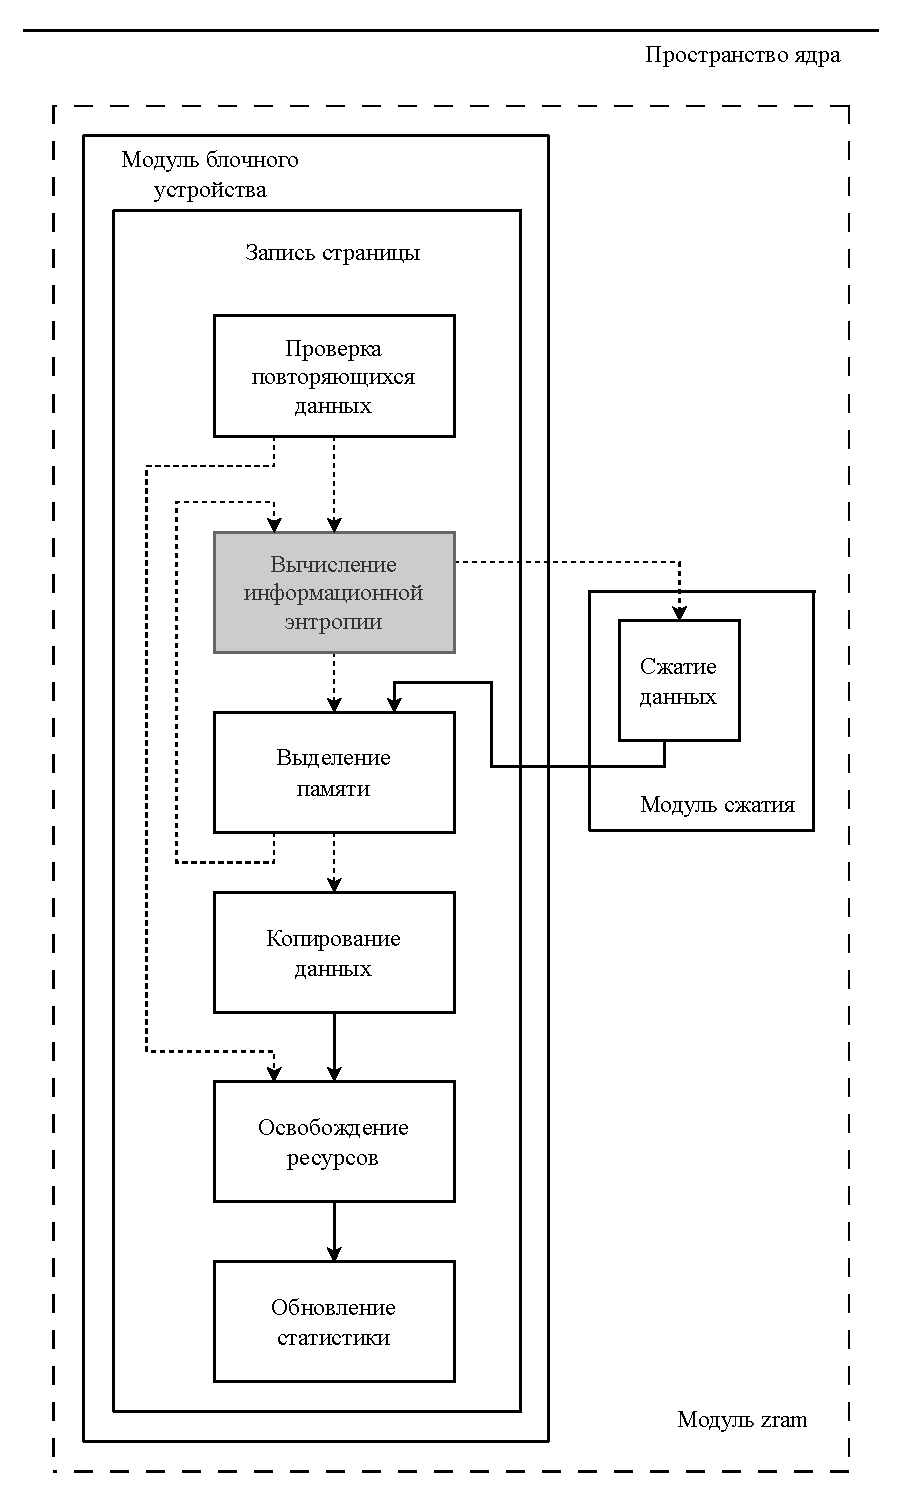
\includegraphics[scale=0.6]{inc/img/structure.pdf}
	\end{center}
	\captionsetup{justification=centering}
	\caption{Структура разрабатываемого программного обеспечения}
	\label{img:structure}
\end{figure}

\section{Выбор типов и структур данных}

Входными и выходными данными является страница памяти, которая задается вектором размером, меньшим или равным размеру страницы в байтах, состоящим из значений от нуля до 255. Поэтому для представления страницы в методе подсчета информационной энтропии должен использоваться массив типа unsigned char размером, равным размеру страницы в байтах.

При выполнении операций с числами с плавающей точкой в режиме пользователя ядро перехватывает системное прерывание и переходит из режима вычислений с целыми числами в режим с плавающей точкой. Если использовать режим с плавающей точкой в пространстве ядра, необходимо сохранять и восстанавливать состояние регистров с плавающей точкой математического сопроцессора. Вычисления с числами с плавающей точкой в режиме ядра выполнять не рекомендуется \cite{love}. Поэтому для представления числовых величин должен использоваться целочисленный тип данных. 

\section{Описание оптимизации метода сжатия страниц}

В результате анализа исходного кода загружаемого модуля zram \cite{zram-code} и описания этапов разрабатываемой оптимизации метода сжатия страниц памяти была построена схема алгоритма записи страницы на диск, приведенная на рисунке \ref{img:write-page}. Псевдокод данного алгоритма представлен в листинге .

TODO: псевдокод.
TODO: написать про пороговое значение.

На разрабатываемый метод подсчета информационной энтропии накладываются следующие ограничения:

\begin{itemize}
	\item вычисляемое значение может представлять неточное значение информационной энтропии, но должно обладать корреляцией с показателями качества сжатия;
	\item все числовые операнды в методе должны быть целыми числами.
\end{itemize}

Разрабатываемый метод является оптимизацией метода скользящего окна. В методе скользящего окна информационная энтропия вычисляется следующим образом:

\begin{equation}
	H(X) = -\sum_{i = 0}^{255} (p_{i} \cdot \log_{2}p_{i}),
\end{equation}

\begin{figure}[H]
	\begin{center}
		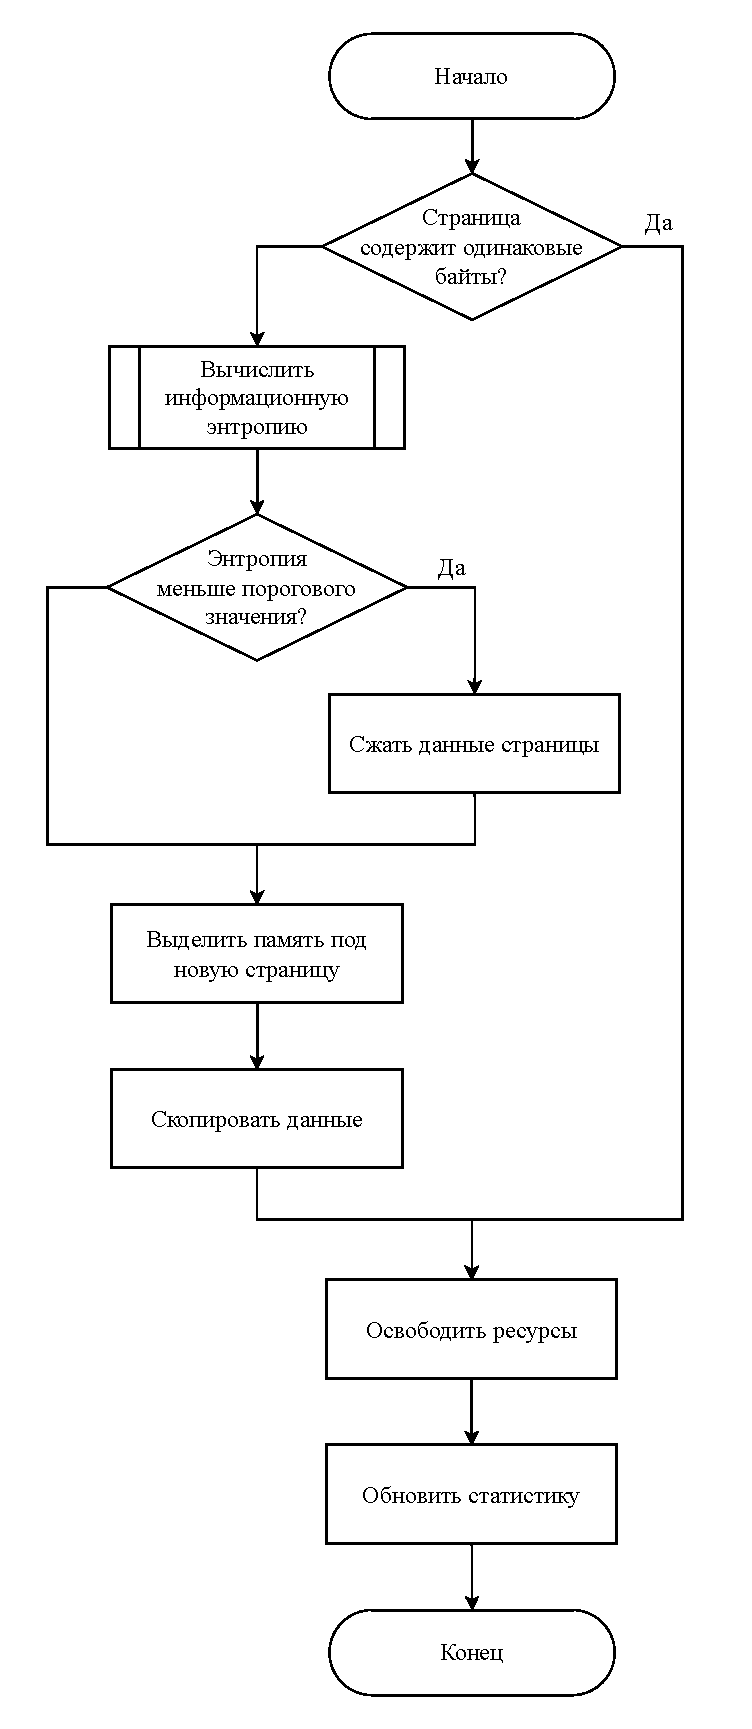
\includegraphics[scale=0.7]{inc/img/write-page.pdf}
	\end{center}
	\captionsetup{justification=centering}
	\caption{Схема алгоритма записи страницы на диск}
	\label{img:write-page}
\end{figure}

\noindentгде $k_{i}$ --- число вхождений значения байта $i$ в массив байтов, представляющий входную страницу, $p_{i} = \frac{k_{i}}{N}$ --- вероятность появления байта в массиве байтов, $i = \overline{0, 255}$, $N$ --- размер страницы в байтах.

Тогда:

\begin{equation}
	H(X) = -\sum_{i = 0}^{255} (\frac{k_{i}}{N} \cdot \log_{2}\frac{k_{i}}{N}).
\end{equation}

В соответствии со свойством логарифма частного можно записать:

\begin{equation}
	H(X) = -\sum_{i = 0}^{255} (\frac{k_{i}}{N} \cdot (\log_{2}k_{i} - \log_{2}N)) = \sum_{i = 0}^{255} (\frac{k_{i}}{N} \cdot (\log_{2}N - \log_{2}k_{i})).
\end{equation}

Так как все числовые операнды являются целыми числами, при определении $p_{i}$ выполняется целочисленное деление и вычисляемое значение округляется. Для сохранения большей точности результатом разрабатываемого метода будет является значение информационной энтропии, умноженное на размер страницы:

\begin{equation}
	H'(X) = N \cdot H(X) = \sum_{i = 0}^{255} (k_{i} \cdot (\log_{2}N - \log_{2}k_{i})),
\end{equation}

Для сокращения времени вычисления логарифма числа вхождений значения байта $i$ в массив байтов по основанию два в разрабатываемом методе используется дополнительный массив размером $log_{2}N$, для которого верно следующее: 

\begin{itemize}
	\item индекс элемента $j$ является целым значением логарифма числа вхождений значения байта $i$, $j = \overline{log_{2}1, log_{2}N}$;
	\item значение элемента с индексом $j$ является наибольшим целым числом $x$ таким, что $log_{2}x = j$.
\end{itemize}

Для определения $\log_{2}k_{i}$ необходимо взять индекс первого элемента описанного массива, который больше или равен $k_i$.

Псевдокод алгоритма разрабатываемого метода подсчета информационной энтропии показан в листинге . Соответствующая ему схема алгоритма приведена на рисунке \ref{img:get-entropy}.

TODO: псевдокод.

\begin{figure}[H]
	\begin{center}
		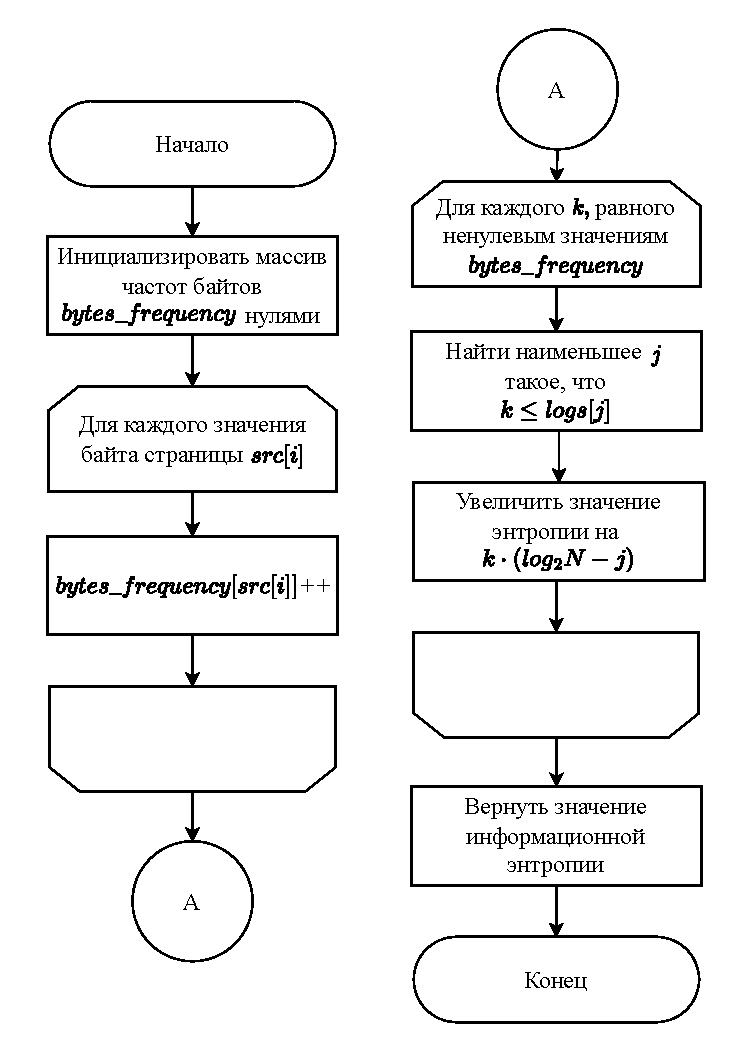
\includegraphics[scale=0.7]{inc/img/get-entropy.pdf}
	\end{center}
	\captionsetup{justification=centering}
	\caption{Схема алгоритма подсчета информационной энтропии}
	\label{img:get-entropy}
\end{figure}

\section{Проектирование тестирования программного обеспечения}

Разрабатываемое программное обеспечение выполняется при записи данных на диск zram. Поэтому для тестирования программного решения необходимо моделировать процесс загрузки страниц памяти на диск. Проверка и отладка разрабатываемого программного обеспечения должны проводиться с помощью ручного тестирования. 

Для проведения тестирования выделены следующие классы эквивалентности:

\begin{enumerate}
	\item Несжимаемые страницы памяти;
	\item Сжимаемые страницы памяти.
\end{enumerate}

Несжимаемыми страницами памяти являются страницы с высоким значением информационной энтропии. В разделе \ref{relation} было доказано, что энтропия сжатых данных выше энтропии исходных данных. Поэтому тестовый набор для первого класса эквивалентности должен включать сжатые данные. Примерами таких данных являются файлы форматов .jpg и .pdf \cite{formats}.

Сжимаемыми страницами памяти являются страницы данных с выделяемой структурой, как было сказано в разделе \ref{relation}. Примерами таких данных являются файлы форматов .c, .h и бинарные файлы \cite{good-compression}, из которых должен состоять тестовый набор для второго класса эквивалентности.

В результате каждого теста должна быть получена статистика сжатия тестового набора, включающая в себя следующую информацию:

\begin{itemize}
	\item объем исходных данных в байтах и страницах;
	\item объем сжатых данных в байтах и страницах;
	\item число несжимаемых страниц;
	\item число страниц с одинаковыми байтами.
\end{itemize}

Система для выполнения тестирования включает следующие компоненты:

\begin{itemize}
	\item персональный компьютер, который является хостом;
	\item виртуальная машина, на которой загружен модуль zram без разрабатываемой оптимизации;
	\item виртуальная машина, на которой загружен модуль zram с разрабатываемой оптимизацией.
\end{itemize}

Тестирование разрабатываемого программного обеспечения состоит из следующих этапов:

\begin{enumerate}
	\item Загрузить тестовый набор с хоста на диск zram виртуальной машины с работающим без разрабатываемой оптимизации модулем zram.
	\item Получить статистику выполнения предыдущего шага.
	\item Загрузить тестовый набор с хоста на диск zram виртуальной машины с работающим с разрабатываемой оптимизации модулем zram.
	\item Получить статистику выполнения предыдущего шага.
	\item Сравнить полученные статистики.
\end{enumerate}

Схема тестирующей системы показана на рисунке \ref{img:testing-scheme}.

\includeimage
    {testing-scheme}
    {f}
    {h}
    {0.5\textwidth}
    {Схема системы для тестирования}

\section*{Вывод}

В данном разделе были разработаны основные этапы оптимизации метода сжатия страниц памяти с использованием подсчета информационной энтропии. Их описание было приведено в виде псевдокода и схем алгоритмов. Были сформулированы требования к разрабатываемому программному решению. Взаимодействие компонентов системы было представлено в виде структуры программного обеспечения. Был обоснован выбор целочисленного типа данных и массива в качестве структуры, представляющей страницу памяти. Были выделены классы эквивалентности, описаны тестовые наборы для ручного тестирования, получаемая в результате статистика и тестирующая система.
